% Source : http://tex.stackexchange.com/questions/40028/highlight-elements-in-the-matrix

\documentclass{article}
	\usepackage{tikz}
	\usetikzlibrary{matrix}

\begin{document}

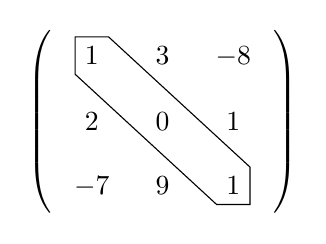
\begin{tikzpicture}
	\matrix[
		matrix of math nodes,
		left delimiter = (,right delimiter = ),
		row sep=10pt,
		column sep = 10pt
	] (m) {
		1  & 3 & -8  \\
		2  & 0 & 1   \\
		-7 & 9 & 1   \\
	};

	\draw (m-1-1.north west) 
		  -- (m-1-1.south west)
		  -- (m-3-3.south west)
		  -- (m-3-3.south east)
		  -- (m-3-3.north east)
		  -- (m-1-1.north east)
		  -- cycle;
\end{tikzpicture}

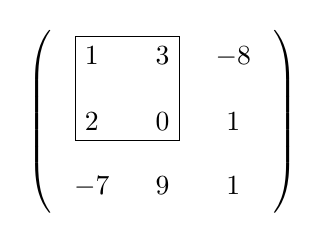
\begin{tikzpicture}
	\matrix[
		matrix of math nodes,
		left delimiter = (,right delimiter = ),
		row sep=10pt,
		column sep=10pt
	] (m) {
		1  & 3 & -8  \\
		2  & 0 & 1   \\
		-7 & 9 & 1   \\
	};

	\draw (m-1-1.north west)
		  -- (m-2-1.south west)
		  -- (m-2-2.south east)
		  -- (m-1-2.north east)
		  -- cycle;
% The previous can be replaced by :
%	\draw (m-1-1.north west)
%		  rectangle (m-2-2.south east);
\end{tikzpicture}

\end{document}
